\documentclass{book}
% Configuration
%----------------
%   Imports
%----------------
\usepackage{xparse}
\usepackage{sectsty}
\usepackage[dvipsnames]{xcolor}
\usepackage{amsmath,amssymb,amsfonts,latexsym,cancel,amsthm,mathtools}


% \setlength{\parindent}{0cm}
% \setlength{\parskip}{5pt}

%-----------------
%   Colours
%-----------------
\definecolor{thmbg}{HTML}{F2F2F9}
\definecolor{lemmabg}{HTML}{FFFAF8}
\definecolor{lemmafr}{HTML}{983b0f}
\definecolor{propbg}{HTML}{f2fbfc}
\definecolor{propfr}{HTML}{191971}
\definecolor{myp}{RGB}{197, 92, 212}
\definecolor{primary}{HTML}{207ba5}    % Main colour
\definecolor{grey17}{RGB}{17, 17, 17}
\definecolor{greybg}{RGB}{249, 249, 249}
\definecolor{MyGrey}{HTML}{5B5B5B}

\definecolor{LightBlue}{rgb}{0.0, 0.64, 1.0}
\definecolor{LightRed}{rgb}{1.0, 0.50, 0.50}
\definecolor{DarkGreen}{rgb}{0.31, 0.54, 0.30}

%----------------
%	Text Styles
%----------------

\DeclareTextFontCommand{\term}{\color{orange}\itshape}
\DeclareTextFontCommand{\bred}{\color{red}\bfseries}
\DeclareTextFontCommand{\itblue}{\color{LightBlue}\itshape}

%----------------
%   URL Colour
%----------------
\usepackage[colorlinks=true]{hyperref}
\hypersetup{
    colorlinks=true,
    linkcolor=black,
    filecolor=magenta,
    urlcolor=blue,
}

%----------------
%   Boxes
%----------------

\usepackage[most]{tcolorbox}

\newcommand\fancybox[3]{%
    \tcbset{
        mybox/.style={
                enhanced,
                boxsep=0mm,
                opacityfill=0,
                overlay={
                        \coordinate (X) at ([xshift=-1mm, yshift=-1.5mm]frame.north west);
                        \node[align=right, text=#1, text width=2.5cm, anchor=north east] at (X) {\bf#2};
                        \draw[line width=0.5mm, color=#1] (frame.north west) -- (frame.south west);
                    }
            }
    }
    \begin{tcolorbox}[mybox]
        #3
    \end{tcolorbox}
}

\tcbuselibrary{theorems,skins,hooks}
\NewDocumentCommand\thmbox{m O{\Large #1} O{greybg} O{primary} O{number within=section}}
{
    \newtcbtheorem[#5]{#1}{\large #2}
    {%
        enhanced
        ,breakable
        ,colback = #3
        ,frame hidden
        ,boxrule = 0sp
        ,borderline west = {2pt}{0pt}{#4}
        ,sharp corners
        ,detach title
        ,before upper = \tcbtitle\par\smallskip
        ,coltitle = #4
        ,fonttitle = \bfseries
        % ,description font = \mdseries
        ,separator sign none
        ,segmentation style={solid, #4}
    }
    {th}
}

\thmbox{Corollary}[Corollary][myp!10][myp!85!black]
\thmbox{Lemma}[Lemma][lemmabg][lemmafr]
\thmbox{Propo}[Preposition][propbg][propfr]
\thmbox{defi}[Definition][primary!12][primary]
\thmbox{Notation}[Notation][white][grey17][no counter]
\thmbox{Theorem}[Theorem][primary!12][primary]

%---------------
%   Commands
%---------------
\newcommand{\theorem}[2]{\begin{Theorem}{#1}{}#2\end{Theorem}}
\newcommand{\corollary}[2]{\begin{Corollary}{#1}{}#2\end{Corollary}}
\newcommand{\lemma}[2]{\begin{Lemma}{#1}{}#2\end{Lemma}}
\newcommand{\proposition}[2]{\begin{Propo}{#1}{}#2\end{Propo}}
\newcommand{\notation}[2]{\begin{Notation}{#1}{}{\em\color{MyGrey}#2}\end{Notation}}
\newcommand{\definition}[2]{\begin{defi}{#1}{}#2\end{defi}}
\newcommand{\demonstration}[1]{\begin{proof}[\color{primary}\textbf{Demonstration.}] #1 \end{proof}}

\theoremstyle{definition}
\newtheorem*{exam}{\color{primary}Example}
\newcommand{\example}[1]{\begin{exam}#1\end{exam}}

\theoremstyle{definition}
\newtheorem*{solu}{\color{primary}Solution}
\newcommand{\solution}[1]{\begin{solu}#1\end{solu}}

\renewcommand{\qed}{\hfill$\blacksquare$}

%---------------
%   Lists
%---------------
\usepackage{tikz}

\usepackage{enumitem}

\newcommand{\cnumero}[2]{
    \tikz[baseline=(myanchor.base)]
    \node[minimum size=0.2cm,circle,
        inner sep=1pt,draw, #2,thick,fill=#2](myanchor)
    {\color{white}\bfseries\fontsize{8}{8}#1};}

\newcommand*{\itembolasazules}[1]{\protect\cnumero{#1}{primary}}

\newcommand{\listo}[1]{
    \begin{enumerate}[label=\itembolasazules{\arabic*}]
        #1
    \end{enumerate}
}

\newcommand{\listu}[1]{
    \begin{itemize}[label=$\color{primary} \bullet$]
        #1
    \end{itemize}
}

%-------------------------
% Table of Contents
%-------------------------

\usepackage{blindtext}
\usepackage{framed}
\usepackage{titletoc}
\usepackage{etoolbox}

\patchcmd{\tableofcontents}{\contentsname}{\contentsname}{}{}

\renewenvironment{leftbar}
{\def\FrameCommand{\hspace{6em}%
        {\color{primary}\vrule width 2pt depth 6pt}\hspace{1em}}%
    \MakeFramed{\parshape 1 0cm \dimexpr\textwidth-6em\relax\FrameRestore}\vskip2pt%
}
{\endMakeFramed}

\titlecontents{chapter}[0em]
{\vspace*{2\baselineskip}}
{\parbox{4.5em}{%
        \hfill\Huge\bfseries\color{primary}\thecontentslabel}%
    \vspace*{-2.3\baselineskip}\leftbar\textbf{\color{primary}\small\chaptername~\thecontentslabel}\\
}{}{\endleftbar}

\titlecontents{section}[8.4em]
{\contentslabel{3em}}{}{}
{\hspace{0.5em}\nobreak\itshape\color{primary}\contentspage}

\titlecontents{subsection}[8.4em]
{\contentslabel{3em}}{}{}
{\hspace{0.5em}\nobreak\itshape\color{primary}\contentspage}

%-----------------------------
%   Chapter formats
%-----------------------------

%==================
% Chapters
%==================
\newtcolorbox{titlecolorbox}[1]{ %the box around chapter
    coltext=white,
    colframe=primary,
    colback=primary,
    boxrule=0pt,
    arc=0pt,
    notitle,
    width=4.8em,
    height=2.4ex,
    before=\hfill
}

\usepackage[explicit]{titlesec}

\makeatletter
\let\old@rule\@rule
\def\@rule[#1]#2#3{\textcolor{primary}{\old@rule[#1]{#2}{#3}}}
\makeatother

\titleformat{\chapter}[display]
{\Huge}
{}
{0pt}
{\begin{titlecolorbox}{}
        {\large\MakeUppercase{\bf\chaptername}}
    \end{titlecolorbox}
    \vspace*{-3.19ex}\noindent\rule{\textwidth}{0.4pt}
    \parbox[b]{\dimexpr\textwidth-4.8em\relax}{\raggedright\MakeUppercase{#1}}{\hfill\fontsize{70}{60}\selectfont{\color{primary}\thechapter}}
}
[]

\titleformat{name=\chapter,numberless}[display]
{\Huge}
{}
{0pt}
{
    \vspace*{-3.19ex}\noindent\rule{\textwidth}{0.4pt}
    \parbox[b]{\dimexpr\textwidth-4.8em\relax}{\raggedright\MakeUppercase{#1}}
}
[]

%==============
% Sections
%==============

\titleformat{\section}[hang]{\Large\bfseries}%
{\rlap{\color{primary}\rule[-6pt]{\textwidth}{0.4pt}}\colorbox{primary}{%
        \raisebox{0pt}[13pt][3pt]{ \makebox[60pt]{% height, width
                \selectfont\color{white}{\thesection}}
        }}}%
{15pt}%
{ \color{primary}#1
    %
}
\titlespacing*{\section}{0pt}{3mm}{5mm}

%================
% Sub sections
%================
\subsectionfont{\Large\color{primary}}


%-----------------
%	BIBLIOGRAPHY AND INDEX
%-----------------

\usepackage{csquotes}
\usepackage[style=alphabetic,citestyle=numeric,sorting=nyt,sortcites=true,autopunct=true,autolang=hyphen,hyperref=true,abbreviate=false,backref=true,backend=biber,defernumbers=true]{biblatex}
\addbibresource{./bibliography.bib} % BibTeX bibliography file
\defbibheading{bibempty}{}

\usepackage{calc} % For simpler calculation - used for spacing the index letter headings correctly
\usepackage{makeidx} % Required to make an index
\makeindex % Tells LaTeX to create the files required for indexing

%---------------------
% Front page
%---------------------
\usetikzlibrary{ shapes.geometric }
\usetikzlibrary{calc}
\usepackage{anyfontsize}
\newcommand{\portada}[3]{
    \begin{tikzpicture}[remember picture,overlay]
        %%%%%%%%%%%%%%%%%%%% Background %%%%%%%%%%%%%%%%%%%%%%%%
        \fill[primary] (current page.south west) rectangle (current page.north east);


        \foreach \i in {2.5,...,22}
            {
                \node[rounded corners,primary!60,draw,regular polygon,regular polygon sides=6, minimum size=\i cm,ultra thick] at ($(current page.west)+(2.5,-5)$) {} ;
            }

        %%%%%%%%%%%%%%%%%%%% Background Polygon %%%%%%%%%%%%%%%%%%%% 
        \foreach \i in {0.5,...,22}
            {
                \node[rounded corners,primary!60,draw,regular polygon,regular polygon sides=6, minimum size=\i cm,ultra thick] at ($(current page.north west)+(2.5,0)$) {} ;
            }

        \foreach \i in {0.5,...,22}
            {
                \node[rounded corners,primary!90,draw,regular polygon,regular polygon sides=6, minimum size=\i cm,ultra thick] at ($(current page.north east)+(0,-9.5)$) {} ;
            }


        \foreach \i in {21,...,6}
            {
                \node[primary!85,rounded corners,draw,regular polygon,regular polygon sides=6, minimum size=\i cm,ultra thick] at ($(current page.south east)+(-0.2,-0.45)$) {} ;
            }


        %%%%%%%%%%%%%%%%%%%% Title %%%%%%%%%%%%%%%%%%%% 
        \node[left,primary!5,minimum width=0.625*\paperwidth,minimum height=3cm, rounded corners] at ($(current page.north east)+(0,-9.5)$)
        {
            {\fontsize{25}{30} \selectfont \bfseries #1}
        };

        %%%%%%%%%%%%%%%%%%%% Subtitle %%%%%%%%%%%%%%%%%%%% 
        \node[left,primary!10,minimum width=0.625*\paperwidth,minimum height=2cm, rounded corners] at ($(current page.north east)+(0,-11)$)
        {
            {\huge \textit{#2}}
        };

        %%%%%%%%%%%%%%%%%%%% Author Name %%%%%%%%%%%%%%%%%%%% 
        \node[left,primary!5,minimum width=0.625*\paperwidth,minimum height=2cm, rounded corners] at ($(current page.north east)+(0,-13)$)
        {
            {\Large \textsc{#3}}
        };

        %%%%%%%%%%%%%%%%%%%% Year %%%%%%%%%%%%%%%%%%%% 
        \node[rounded corners,fill=primary!70,text =primary!5,regular polygon,regular polygon sides=6, minimum size=2.5 cm,inner sep=0,ultra thick] at ($(current page.west)+(2.5,-5)$) {\LARGE \bfseries \the\year{}};

    \end{tikzpicture}
}
\usepackage[letterpaper]{geometry}
\usepackage{graphicx, wrapfig, subcaption, setspace, booktabs}
\usepackage[T1]{fontenc}
\usepackage{babel}
\usepackage[scaled]{helvet}     % Document source
%\renewcommand{\familydefault}{\sfdefault}
\usepackage[utf8]{inputenc}
\usepackage{url, lipsum}
\usepackage{tabularx}

% You can change the main color
% \definecolor{primary}{HTML}{}

\begin{document}

\pagestyle{empty}
\portada{CSC263}{Data Structures and Analysis}{Sinan Li}
\newpage

\tableofcontents

\newpage

\part{Data Structure}

\chapter{Priority Queues and Heaps}

\begin{minipage}[t]{0.45\linewidth}
    \textbf{Data}
    
    \listu{
        \item Collection of elements
    
        \item Each element $x$ has a priority 
        
        $x$.\textit{priority}
    }
\end{minipage}
\begin{minipage}[t]{0.45\linewidth}
    \textbf{Operations}
    
    \listu{
        \item \textsc{Insert}$(Q, x)$
        
        Add $x$ to $Q$ 
        
        Note: $x$.\textit{priority} can be non-unique

        \item \textsc{Max}$(Q)$
        
        Return the element with max priority

        Note: $Q$ is unchanged

        \item \textsc{Extract-Max}$(Q)$
        
        Remove and return the element with the max priority
    }
\end{minipage}

\section{Implementation}

\subsection{Attempts}

\subsubsection{Implementation 1: Unsorted Array / Linked List}

\begin{itemize}
    \item \textsc{Insert} takes $\Theta(1)$ time in the worst case 
    \item \textsc{Max} takes $\Theta(n)$ time in the worst case 
    \item \textsc{ExtractMax} takes $\Theta(n)$ time in the worst case
\end{itemize}

\subsubsection{Implementation 2: Sorted Array / Linked List}

\begin{itemize}
    \item \textsc{Insert} takes $\Theta(n)$ time in the worst case 
    \item \textsc{Max} takes $\Theta(1)$ time in the worst case 
    \item \textsc{ExtractMax} takes $\Theta(1)$ time in the worst case
\end{itemize}

\subsection{Implementation}

We want to combine the advantages of both data structures by having a ``partially sorted'' ADT -- a (binary) \term{heap}\index{Heap}. 

There are two kinds of binary heaps: max-heaps and min-heaps. In both kinds, the values in the nodes satisfy a \bred{heap property}, the specifics of which depend on the kind of heap. 

\begin{itemize}
    \item Max heap property: the key of every node $x$ is \itblue{larger} than or equal to the keys of its children. 
    
    The largest element in a max-heap is stored at the root.
    
    \item Min heap property: the key of every node $x$ is \itblue{smaller} than or equal to the keys of its children
    
    The smallest element in a min-heap is stored at the root,
\end{itemize}

These are called \term{heap orders}. There is no ordering between the siblings. A max/min heap is valid if it is a nearly complete binary tree and it satisfies the max/min heap property.

\begin{figure}[ht!]
    \tikzset{
        every node/.style = {draw, circle, minimum size=2em}, 
        level 1/.style={sibling distance=6em}, 
        level 2/.style={sibling distance=3em}, 
        level 3/.style={sibling distance=1.5em}
    }
    \centering
    \begin{tikzpicture}
        \node {$17$}
        child {
            node {$12$}
            child { node {$5$} }
            child { node {$8$} }
        }
        child {node {$2$} };
    \end{tikzpicture}
    \hfill
    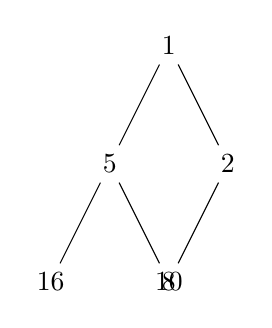
\begin{tikzpicture}
        \node {$1$}
        child {
            node {$5$}
            child { node {$16$} }
            child { node {$8$} }
        }
        child {node {$2$} 
            child { node {$10$} }
            child[missing]
        };
    \end{tikzpicture}
    \hfill
    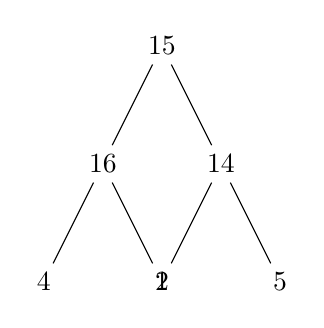
\begin{tikzpicture}
        \node {$15$}
        child {
            node {$16$}
            child { node {$4$} }
            child { node {$2$} }
        }
        child {node {$14$} 
            child { node {$1$} }
            child { node {$5$} }
        };
    \end{tikzpicture}
    \caption{A valid max-heap (left), a valid min-heap (middle), and an invalid heap (right)}
\end{figure}

Although a heap is an \bred{almost complete binary tree} \footnote{That is, the tree is completely filled on all levels except possibly the lowest, which is filled from the left up to a point. }, in practice, we usually use an array to store the data in memory. An array $H$ that represents a heap is an object with two attributes: $H$.\textit{length}, which (as usual) gives the number of elements in the array, and $H$.\textit{heap-size}, which represents how many elements in the heap are stored within array $H$. The root of the tree is $H[1]$, and given the index $i$ of a node, we can compute the indices of its parent, left child, and right child:

\begin{minipage}[t]{0.3\linewidth} \begin{itemize}
    \item \textsc{Parent}
    
    \textbf{return} $\lfloor i / 2 \rfloor$
\end{itemize} \end{minipage}
\begin{minipage}[t]{0.3\linewidth} \begin{itemize}
    \item \textsc{Left}
    
    \textbf{return} $2i$
\end{itemize} \end{minipage}
\begin{minipage}[t]{0.3\linewidth} \begin{itemize}
    \item \textsc{Right}

    \textbf{return} $2i + 1$
\end{itemize} \end{minipage}

\section{Operations}
\subsection{\textsc{Insert}}

To insert element with key $p$ into the heap $H$, 

\listu{
    \item Increment $H$.\textit{heap-size} and add a new node with key $p$ to the next available position

    \item Repeatedly swap the new item with its parent until the heap property is satisfied

    This swapping process is called \bred{bubbling up}

    \item Worst-case runtime: $\Theta(\lg n)$
}

{~~~}

For example, consider \textsc{Insert}$(H, 17)$ where $H = [16, 8, 10, 1, 5, 3]$

\begin{minipage}[t]{0.3\linewidth} \begin{center} 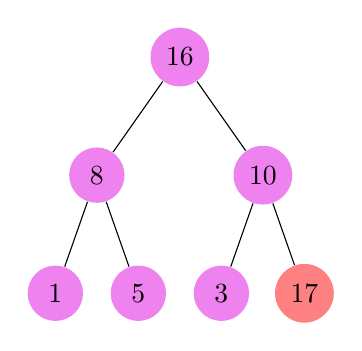
\begin{tikzpicture} [
    every node/.style = {circle, fill=Violet, minimum size=2em}, 
    level 1/.style={sibling distance=6em}, 
    level 2/.style={sibling distance=3em}, 
    level 3/.style={sibling distance=1.5em},
    baseline=(current bounding box.north)
]
    \node {$16$} 
    child {
        node {$8$} 
        child { node {$1$} }
        child { node {$5$} }
    }
    child {
        node {$10$}
        child { node {$3$} }
        child { node [fill=red!50] {$17$} }
    };
\end{tikzpicture} \end{center} \end{minipage}
\begin{minipage}[t]{0.3\linewidth} \begin{center} 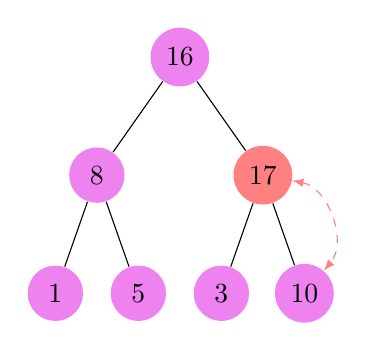
\begin{tikzpicture} [
    every node/.style = {circle, fill=Violet, minimum size=2em}, 
    level 1/.style={sibling distance=6em}, 
    level 2/.style={sibling distance=3em}, 
    level 3/.style={sibling distance=1.5em},
    baseline=(current bounding box.north)
]
    \node {$16$} 
    child {
        node {$8$} 
        child { node {$1$} }
        child { node {$5$} }
    }
    child { 
        node [fill=red!50] (17) {$17$}
        child { node {$3$} }
        child { node (10) {$10$} }
    };

    \draw[bend left=60, dashed,latex-latex,color=red!50]  (17) to (10);
\end{tikzpicture} \end{center} \end{minipage}
\begin{minipage}[t]{0.3\linewidth} \begin{center} 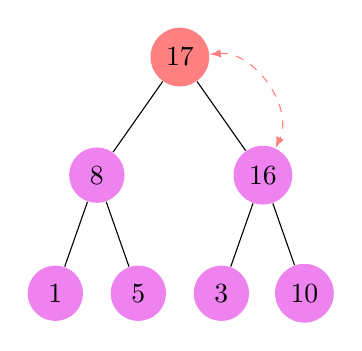
\begin{tikzpicture} [
    every node/.style = {circle, fill=Violet, minimum size=2em}, 
    level 1/.style={sibling distance=6em}, 
    level 2/.style={sibling distance=3em}, 
    level 3/.style={sibling distance=1.5em},
    baseline=(current bounding box.north)
]
    \node [fill=red!50] (17) {$17$}
    child {
        node {$8$} 
        child { node {$1$} }
        child { node {$5$} }
    }
    child { 
        node (16) {$16$}     
        child { node {$3$} }
        child { node {$10$} }
    };

    \draw[bend left=60, dashed,latex-latex,color=red!50]  (17) to (16);
\end{tikzpicture} \end{center} \end{minipage}

{~~~}

{~~~}

{~~~}

\textsc{Max-Heap-Insert}$(H, p)$:

    $i = H.\textit{heap-size} = H.\textit{heap-size} + 1$

    $H[i] = p$

    \textbf{while} $\textsc{Parent}(i) > 0$ \textbf{and} $H[i] > H[\textsc{Parent}(i)]$:

          swap $H[i]$ with $H[\textsc{Parent}[i]]$

          $i = \textsc{Parent}(i)$

\subsection{\textsc{Find-Max}}

\begin{minipage}[t]{0.45\linewidth}
    To find the maximum key in the heap $H$, 

    \listu{
        \item Simply return the item in the root

        \item Worst-case runtime: $\Theta(1)$
    }

    {~~~}

    \textsc{Find-Max}$(H)$
    \begin{enumerate}[label=\arabic*] \setlist{nosep}
        \item {~~~} \textbf{return} $H[1]$
    \end{enumerate}
\end{minipage}%
\begin{minipage}[t]{0.45\linewidth} \begin{center} 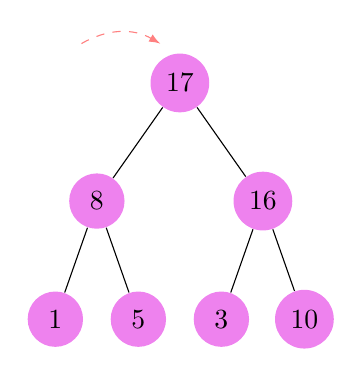
\begin{tikzpicture} [
    every node/.style = {circle, fill=Violet, minimum size=2em}, 
    level 1/.style={sibling distance=6em}, 
    level 2/.style={sibling distance=3em}, 
    level 3/.style={sibling distance=1.5em},
    baseline=(current bounding box.north)
]
    \node (root) {$17$}
    child {
        node {$8$} 
        child { node {$1$} }
        child { node {$5$} }
    }
    child { 
        node (16) {$16$}     
        child { node {$3$} }
        child { node {$10$} }
    };
    
    \draw[bend left=30, dashed, -latex, color=red!50] (-1.25,0.5) to (-0.25,0.5);
\end{tikzpicture} \end{center} \end{minipage}

\part{Analysis}

\end{document}
